\documentclass[a4paper, openany, oneside, 11pt]{book} 
\usepackage[top=3cm, bottom=3cm, left=2.75cm, right=2.75cm]{geometry}

% structure packages
\usepackage{subfiles}
\usepackage[nottoc]{tocbibind}
\usepackage{makeidx} 
	\makeindex
\usepackage{enumitem}
\usepackage{fancyhdr} % fancy headder
	\setlength{\headheight}{15pt}
	\pagestyle{fancy}
	\renewcommand{\chaptermark}[1]{\markboth{#1}{}}
	\renewcommand{\sectionmark}[1]{\markright{#1}{}}
	\fancyhf{}
	\fancyhead[LE,RO]{\thepage}
	\fancyhead[LO]{{\nouppercase{\leftmark}}}
	\fancyhead[RE]{{\nouppercase{\leftmark}}} 
	\fancypagestyle{plain}{
	\fancyhf{} 
	\renewcommand{\headrulewidth}{0pt} 
	\renewcommand{\footrulewidth}{0pt}}

\usepackage{blindtext}
\usepackage{titlesec}
\usepackage{color}
    \definecolor{gray75}{gray}{0.75}
    \titleformat{\chapter}[hang]{\Huge\bfseries}{\thechapter\hspace{15pt}\textcolor{gray75}{$|$}\hspace{15pt}}{0pt}{\Huge\bfseries}

\setcounter{tocdepth}{4}
\setcounter{secnumdepth}{4}

% language settings
\usepackage[english,serbian]{babel}
\usepackage[utf8x]{inputenc} 
\usepackage[OT2,OT1]{fontenc} 
\usepackage[german=quotes]{csquotes}
\DeclareQuoteAlias{dutch}{serbian}

% character conversion settings
\renewcommand{\rmdefault}{wncyr} 
\renewcommand{\sfdefault}{wncyss}
\renewcommand{\encodingdefault}{OT2}

% figures, graphics \& plots
\usepackage[pdftex]{graphicx}
	\graphicspath{{res/}{../res/}}
\usepackage{wrapfig}
\usepackage{rotating}
\usepackage{caption}
\usepackage[list=true,listformat=simple]{subcaption} 
\usepackage{pgfplots}
\usepackage{pgfplotstable}
\usepackage{tikz}
	\usetikzlibrary{calc,patterns,decorations.pathmorphing,decorations.markings}
	\usetikzlibrary{arrows, shapes, calc, positioning}
	\usetikzlibrary{circuits.logic.US}
	\tikzstyle{gnd}=[fill, pattern = north east lines, draw = none, minimum width = 1.00cm, minimum height = 0.05cm]
	\usetikzlibrary{shadings, calc, decorations.markings}
    \tikzset{->-/.style={decoration={
      markings,
      mark=at position #1 with {\arrow{>}}},postaction={decorate}},
      ->-/.default=0.5,
      }
\usepackage{multirow}
\usepackage{pdflscape}
\usepackage{listings}
\usepackage{adjustbox}
\definecolor{codegreen}{rgb}{0,0.6,0}
\definecolor{codegray}{rgb}{0.5,0.5,0.5}
\definecolor{codepurple}{rgb}{0.58,0,0.82}
\definecolor{backcolour}{rgb}{0.95,0.95,0.92}
\lstdefinestyle{mystyle}{
    backgroundcolor=\color{backcolour},   
    commentstyle=\color{codegreen},
    keywordstyle=\color{purple},
    numberstyle=\tiny\color{codegray},
    stringstyle=\color{codepurple},
    basicstyle=\ttfamily\scriptsize,
    breakatwhitespace=false,         
    breaklines=true,                 
    captionpos=b,                    
    keepspaces=true,                 
    numbers=left,                    
    numbersep=5pt,                  
    showspaces=false,                
    showstringspaces=false,
    showtabs=false,                  
    tabsize=2
}
\lstset{style=mystyle}


\usepackage[title]{appendix}

% styles
\usepackage{tcolorbox}
\usepackage{color, colortbl}
\definecolor{Gray}{gray}{0.9}
\usepackage{lipsum}
\usepackage{hyperref} 
	\hypersetup{
	    colorlinks,
	    citecolor=black,
	    filecolor=black,
	    linkcolor=black,
	    urlcolor=blue
	}

% math packages
\usepackage{amsmath} 
\usepackage{amsfonts} 
\usepackage{amssymb} 
\usepackage{mathtools}
\usepackage{cancel}
\usepackage{tikz}
\usetikzlibrary{patterns}
\usepackage[siunitx]{circuitikz}
	\sisetup{output-decimal-marker = {,}}
\usepackage{mhchem}
\tikzset{
    partial ellipse/.style args={#1:#2:#3}{
        insert path={+ (#1:#3) arc (#1:#2:#3)}
    }
}
\def\centerarc[#1](#2)(#3:#4:#5)% Syntax: [draw options] (center) (initial angle:final angle:radius)
    { \draw[#1] ($(#2)+({#5*cos(#3)},{#5*sin(#3)})$) arc (#3:#4:#5); }
 \usepackage{soul}
 
% upright math operators
\DeclareMathOperator{\lin}{lin}
\DeclareMathOperator{\sgn}{sgn}

% chapter localization
\addto\captionsserbian{\renewcommand{\contentsname}{Sadrzhaj}} 
\addto\captionsserbian{\renewcommand{\bibname}{Literatura}}
\addto\captionsserbian{\renewcommand{\indexname}{Indeks pojmova}} 
\addto\captionsserbian{%
  \renewcommand\appendixname{Dodatak}
  \renewcommand\appendixpagename{Dodatak}
}
\setlength{\marginparwidth}{2cm}
\usepackage[]{todonotes}
\renewcommand{\chaptername}{}

\makeatletter
\providecommand*{\diff}%
{\@ifnextchar^{\DIfF}{\DIfF^{}}}
\def\DIfF^#1{%
\mathop{\mathrm{\mathstrut d}}%
\nolimits^{#1}\gobblespace}
\def\gobblespace{%
\futurelet\diffarg\opspace}
\def\opspace{%
\let\DiffSpace\!%
\ifx\diffarg(%
\let\DiffSpace\relax
\else
\ifx\diffarg[%
\let\DiffSpace\relax
\else
\ifx\diffarg\{%
\let\DiffSpace\relax
\fi\fi\fi\DiffSpace}

\bibliographystyle{ieeetr}

\begin{document}

\thispagestyle{empty}

\begin{center}
    \begin{Large}
        Univerzitet u Beogradu -- Elektrotehnichki fakultet \\ \vspace{5pt}
    \end{Large}
\end{center}

\vspace{100pt}
\begin{center}
	\begin{huge} \textbf{MASTER RAD} \end{huge} \\ 
        \vspace{10pt}
        na temu \\
        \vspace{10pt}
    \begin{huge} 
        \textbf{Sinteza video zapisa} \\ \vspace{-2pt}
        \textbf{na osnovu govornog signala upotrebom} \\ \vspace{-2pt}
        \textbf{rekurentnih neuralnih mrezha} \\
    \end{huge} 
\end{center}
\vspace{200pt}
\begin{center}
	\begin{large}
		kandidat: \hfill  mentor: \\ \vspace{5pt}
		Veljko Sheshelj, 3253/2018 \hfill doc. dr Predrag Tadic1
	\end{large}
\end{center}
\vfill
\begin{center}	
avgust, 2020.
\end{center}

\chapter*{Zahvalnica}
% \addcontentsline{toc}{chapter}{Zahvalnica}

\newpage
\tableofcontents

\newpage
\listoffigures
\chapter*{Uvod} 
\addcontentsline{toc}{chapter}{Uvod}
\markboth{Uvod}{Uvod}


\chapter{Obelezhja govora}
Prvi korak u sintezi lazhnog videa iz govora je odredjivanje karakteristichnih obelezhja govornog signala. Komponentne audio signala treba da su dovoljno dobre da nose lingvistichku komponentu, ali i da su otporne na pozadinski shum i na ostale smetnje.
Jedna od osnovnih pretpostavki vezanih za obradu govornog signala jeste da se govor mozhe prikazati kao izlaz linearnog, vremenski promenljivog sistema, chija se svojstva sporo menjaju sa vremenom. To vodi ka osnovnom principu analize govora koji kazhe da ako se posmatraju dovoljno kratki segmenti govornog signala, da se tada svaki segment mozhe modelirati kao izlaz linearnog, vremenski invarijantnog sistema \cite{OPGpredavanja}. Stoga se kratki segmenti govora mogu opisati konvolucionom jednachinom
\begin{equation}\label{eq:1.1}
s(t) = e(t)*\theta(t)
\end{equation}
pri chemu $s(t)$ predstavlja rezultatni govorni signal, $e(t)$ predstavlja pobudnu vazdushnu struju (eksitaciju) i $\Theta(t)$ impulsni odziv organa govornog trakta. U rachunarskoj obradi govora, signale je zgodnije posmatrati u diskretnom domenu
\begin{equation}
s[n] = e[n]*\theta[n]
\end{equation}
Zavisno od tipa eksitacije, govorni glasovi (fonemi) se mogu podeliti u tri distinktne kategorije:
\begin{itemize}[noitemsep]
\item zvuchni glasovi
\item frikativi (bezvuchni glasovi)
\item plozivi
\end{itemize}
Kod zvuchnih glasova, vazduh prelazi preko zategnutih glasnih zhica koje po\-chinju da vibriraju relaksiranim oscilacijama, proizvodec1i kvazi-periodichne chetvrtke koje c1e pobuditi vokalni trakt. Tipichni predstavnici zvuchnih glasova su samoglasnici. Pobuda koja proizvodi frikative je okarakterisana shirokim spektralnim sadrzhajem kao shto je sluchajni shum (glas \enquote{sh}). Plozivi nastaju pobudom koja je visokog inteziteta i kratkog trajanja (poput Dirakovog impulsa) (glasovi \enquote{b}, \enquote{p}, \enquote{t}...). Promenom oblika vokalnog trakta menja se frekvencijski sadrzhaj pobude i kao rezultat se dobijaju razlichiti fonemi. Engleski jezik razlikuje 42 fonema.\\
Problem govorne analize predstavlja odredjivanje parametara eksitacije i parametara implusnog odziva vokalnog trakta. Ovaj problem se mozhe nazvati i problemom razdvajanja konvolucionih komponenti, shto je poznato pod nazivom dekonvolucija.

\section{Kepstrum}
Kepstrum diskretnog signala $s[n]$ se mozhe izrachunati pomoc1u formule \cite{kepstri}
\begin{equation}
c_s[n] = \boldsymbol{\mathcal{F}^{-1}}(\log(|\boldsymbol{\mathcal{F}}(s[n])|)
\end{equation}
gde su sa $\boldsymbol{\mathcal{F}}$ i $\boldsymbol{\mathcal{F}^{-1}}$ oznachene diskretna Furijeova transformacija (DFT) i inverzna DFT. Primenom DFT na jednachinu \ref{eq:1.1} dobija se
\begin{equation}
S(f) = E(f)\cdot\Theta(f)
\end{equation}
Izrachunavanje kepstruma mozhe se smatrati sistemom za dekonvoluciju zbog chinjenice da logaritam proizvoda dve komponetne predstavlja zbir logaritmovanih komponenti
\begin{align}
\log|S(f)| &= \log|E(f)\cdot\Theta(f)|\\
           &= \log|E(f)| + \log|\Theta(f)|\\
           &= C_E(f)+ C_{\Theta}(f)
\end{align}
Primenom inverzne Furijeove transformacije dobija se kepstrum govornog signala
\begin{align}
c_s[n] &= \boldsymbol{\mathcal{F}^{-1}}(C_E(f)+ C_{\Theta}(f))\\
       &= \boldsymbol{\mathcal{F}^{-1}}(C_E(f))+
       	  \boldsymbol{\mathcal{F}^{-1}}(C_{\Theta}(f))\\
       &= c_e[n]+ c_{\theta}[n]
\end{align}
U obliku signala $c_s[n]$ uochljive su oblasti u kojima dominiraju ekvivalenti vazdushne pobude  $c_e[n]$, odnosno impulsnog odziva govornih organa $c_{\theta}[n]$. Uticaj vazdushne pobude dominantniji je pri vec1im vrednostima argumenta, dok nizhe vrednosti argumenta nose informaciju o impulsnom odzivu vokalnog trakta. Zbog toga se najchesh\-c1e koristi prvih 12 kepstralnih koeficijenata, dok nulti koeficijent nosi informaciju o energiji signala.\\
Poshto je govor realan signal, amplituda spektra $|S(f)|$ je parna funkcija i kepstrum c1e imati realne vrednosti
\begin{align}
c_s[n] &= \boldsymbol{\mathcal{F}^{-1}}(\log(|\boldsymbol{\mathcal{F}}(s[n])|)\\
&=\frac{1}{N}\sum^{N-1}_{k=1}\log(|\boldsymbol{\mathcal{F}}(s[n])|)e^{\frac{j2kn\pi}{N}}\\
&=\frac{1}{N}\sum^{N-1}_{k=1}\log(|\boldsymbol{\mathcal{F}}(s[n])|)(\cos\left(\frac{2kn\pi}{N}\right)+j\sin\left(\frac{2kn\pi}{N}\right))\\
&=\frac{1}{N}\sum^{N-1}_{k=1}\log(|\boldsymbol{\mathcal{F}}(s[n])|)\cos\left(\frac{2kn\pi}{N}\right)
\end{align}
Zbog ovog svojstva, chesto se umesto inverzne diskretne Furijeove transoformacije koristi diskretna kosinusna transformacija radi smanjenja kompleksnosti izrachunavanja.

\section{Mel-frekvencijski kepstralni koeficijenti}
Prethodno opisani postupci se chesto koriste u primenama vezanim za automat\-sko prepoznavanje govora. U cilju oponashanja ljudskog nachina dozhivljavanja razlichitih uchestanosti u fonetima i primenjujuc1i kepstralnu analizu nastaju Mel-frekvencijski kepstralni koeficijnti (MFKK). 
\subsection{Melova frekvencijska skala}
Mel-skala je uskladjena sa ljudskim osec1ajem visine glasa odnosno njegove uchestanosti. Njeno dobijanje se vrshi eksperimentalno, slushaocu se reprodukuje ton uchestanosti $\SI{1000}{Hz}$ i kao njegovo zapazhanje o visini ovog tona se belezhi vrednost $\SI{1000}{mel}$, i ova vrednost se koristi kao mera uporedjivanja za dalje dobijanje mel skale. Zatim se uchestanost povec1ava sve dok slushalac ne primeti ton koji slusha ima duplo vec1u visinu od uporedne vrednosti i ta visina oznachava vrednosh\-c1u od $\SI{2000}{mel}$. Ovaj se princip dobija za dobijanje ostalih vrednosti skale. Eksperimenti su ipak pokazali da je medjusobna zavisnost mela i herca lienarna do $\SI{500}{Hz}$, dok iznad ove uchestanosti jednakim promenama mela odgovara sve vec1a promena u hercima. Za konvertovanje frekvencije u melovu skalu i nazad mogu se koristiti formule
\begin{equation}\label{freq2mel}
M(f) = 1125\log\left(1+\frac{f}{700}\right)
\end{equation}
\begin{equation}\label{mel2freq}
M^{-1}(m) = 700\left(\exp\left(\frac{m}{1125}\right)-1\right)
\end{equation}
\begin{figure}[h!]
\centering
  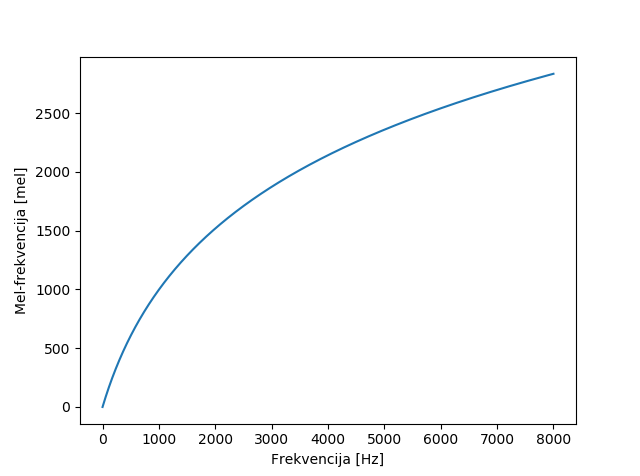
\includegraphics[scale=0.8]{res/freq2mel.png}
  \caption{Mel-frekvencijska skala}
  \label{fig:1}
  \vspace{0pt}
\end{figure}
\subsection{Melova banka filtara}
Postojanje auditornih kritichnih opsega je takodje osobina koja uslovljava ljudski dozhivljaj razlichitih uchestanosti. Ova pojava vezana je za chujni dozhivljaj slushaoca  prilikom slushanja dva razlichita tona na razlichitim uchestanostima. Dakle, ukoliko se slushocu pusti ton uchestanosti $f_1$ koja se nalazi u nekom chujnom opsegu, tada slushalac ima dozhivljaj tona u skladu sa mel sklaom. Ukoliko se pored tog tona pusti drugi ton uchestanosti $f_2$ tada zvuchni dozhivljaj slushaoca zavisi od medjusobne frekventne bliskosti ova dva tona. Naime, ukoliko je frekventni razmak dovoljno mali tako da se nalaze unutar istog kritichnog chujnog opsega dolazi do pojave maskiranja i slushalac chuje ton $f_1$, ali vec1e glasnosti. Ukoliko je frekventni razmak ovih tonova vec1i od shirine chujnog kritichnog opsega tada slushalac chuje dva tona na odgovarajuc1im prethodno pomenutim uchestanostima. Imajuc1i to u vidu frekvencijski opseg govornog signala potrebno je izdeliti na opsege. Ti opsezi formiraju melovu banku filtara. Postupak formitanja melove banke filtara se mozhe izdeliti na korake:
\begin{enumerate}
\item Koristec1i jendachinu \ref{freq2mel} konvertovati donju i gornju granicu govornog signala u melovu skalu. Za donju granicu se mozhe uzeti vrednost od $\SI{0}{Hz}$, dok je gornja frekvencija obichno uslovljena Nikvistovim kreiterijumom. U korish\-c1enom skupu podataka, govrni signal je odabiran sa $\SI{16}{kHz}$, pa je za gornju granicu korish\-c1ena vrednost od $\SI{8}{kHz}$.
\item Izdeliti opseg govornog signala na melovoj skali na ekvidistantne delove (opsege). Za broj delova se obichno uzima broj iz intervala $[26,\ 40]$. Za $n$ filtara dobijaju se $n+2$ frekvencije na melovoj skali.
\item Dobijene melove frekvencije, potrebno je vratiti u $\SI{}{Hz}$ frekvencije, formulom \ref{mel2freq}, koje se kasnije koriste za centralne uchestanosti trougaonih filtara
\end{enumerate}
\begin{figure}[h!]
\centering
  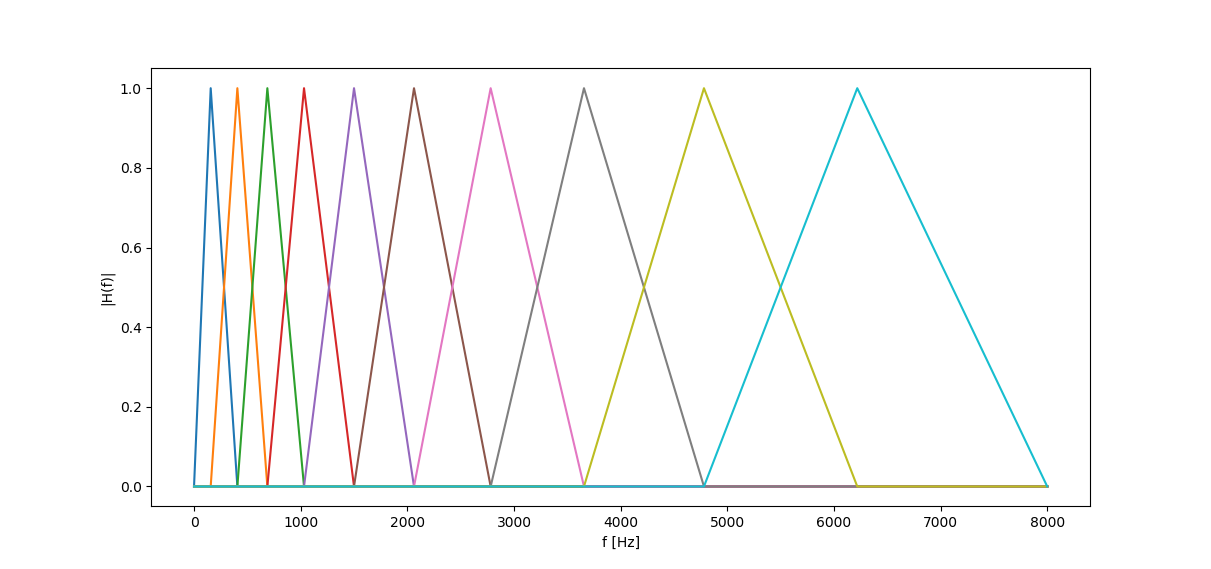
\includegraphics[scale=0.5]{res/10filterbank.png}
  \caption{Govorni frekvencijski opseg podeljen na 10 mel filtara}
  \label{fig:2}
  \vspace{0pt}
\end{figure}
\subsection{Algoritam izrachunavanja MFKK}
U ovom poglavlju c1e biti prikazan detaljan postupak dobijanja MFKK.
\begin{itemize}
\item \textbf{Visokofrekventno filtriranje}\\
Govorni signal je po prirodi analogni signal, koji je potrebno diskretizovati i digitalizovati da bi se izrachunala trazhena obelezhja. Pomenuti procesi su niskofrekventni i utichu na slabljenje vishih spektralnih komponenti u govornog signalu. Iz tog razloga nakon izvrshene digitalizacije, a pre samog izdvajanja obelezhja, potrebno je izvrshiti predobradu snimljenog govornog signala. To se postizhe primenom visokopropusnog filtra prvog reda
\begin{equation}
H(z) = 1-az^{-1}
\end{equation}
pri chemu se parametar $a$ bira iz intervala $[0.95,\ 0.98] $\cite{kepstrum}.
\item \textbf{Prozorovanje signala}\\
Na pochetku poglavlja je recheno da se samo kratki segmenti govora mogu smatrati kao izlaz linearnog, vremenski invarijantnog sistema. Sa tim u vezi signal je potrebno izdeliti na prozore duzhine $\SI{20}{ms}-\SI{40}{ms}$  \cite{OPGpredavanja}. U ovom radu izabrana je duzhina prozora od $\SI{25}{ms}$, sa preklapanjem izmedju susdenih prozora od $\SI{15}{ms}$. Naredni koraci se primenjuju za svaki prozor.
\item \textbf{Izrachunavanje spektra snage}\\
Za svaki prozor govornog signala je prvobitno potrebno odrediti DFT. Radi potiskivanja bochnih lobova, zgodno je primeniti Hamingov prozor pre izrachunavanja DFT. U ovom radu DFT se izrachunava u 512 tachaka. Spektar snage se mozhe estimirati periodogramom, koji za signal $s[n]$ se izrachunava po formuli
\begin{align}
S(f) &=\boldsymbol{\mathcal{F}}(s[n])\\
P(f) &=\frac{1}{N}|S(f)|^2
\end{align}
\item \textbf{Filtriranje spektra snage melovom bankom filtara}\\
Dobijeni periodogram je potrebno filtrirati kroz svaki filtar iz melove banke. Dobijeni koeficijenti za svaki filtar se sumiraju. Na kraju se dobijaju koeficijenti koji nam govore koliko je energije sadrzhano u svakom filtru filter banke.
\item \textbf{Logaritmovanje}\\
Logaritmovati svaki koeficijent dobijen propushtanjem periodograma kroz banku filtara.
\item \textbf{Diskretna kosinusna transformacija}\\
Diskretnom kosinusnom transformacijom nad logaritmovanim energijama dobijaju se kepstralni koeficijenti.
\end{itemize}
\subsection{Dinamichka obelezhja}
Chesto je od interesa posmatrati i promenu MFKK u vremenu \cite{kepstrum}. Na ovaj nachin, korish\-c1ena obelezhja direktno nose informaciju o promenama izmedju susednih prozora govornog signala. Radi izrachunavanja ovih obelezhja koriste se polinomijalne aproksimacije prvog i drugog izvoda kepstralnih koeficijenata \cite{MFKKlink}
\begin{align}
\Delta c_t &= \frac{\sum^{N}_{n=1}n(c_{t+n}-c_{t-n})}{2\sum^{N}_{n=1}n^2}\\
\Delta^2 c_t &= \frac{\sum^{N}_{n=1}n(\Delta_{t+n}-\Delta_{t-n})}{2\sum^{N}_{n=1}n^2}
\end{align}
gde su $\Delta c_t$ i $\Delta^2 c_t $ delta i delta-delta kepstralni koeficijenti za prozor $t$, izrachunati iz statichkih kepstralnih koeficijenata iz okolnih prozora. Tipichna vrednost koja se uzima je $N=2$.
\section{Prikaz obelezhja govora}
U ovom radu, kao vektor ulaznih parametara, korish\-c1eno je 13 kepstralnih koeficijenata, sa njihom deltama, shto daje ulazni vektor dimenzije 26. Umesto prvog kepstra, korish\-c1ena je energija signala. Iz baze video fajlova, samo audio snimci su izvucheni uz pomoc1 alata $FFmpeg$ \cite{FFmpeg}, chime se dobija baza audio snimaka govora predsednika Obame. Nakon toga, svaki video je normalizovan uz pomoc1 $FFmpeg-normalize$ dodatka \cite{FFmpegN}. Prikaz nekih kepstralnih koeficijenata, za nasumichno odabran audio snimak iz baze, se mozhe pogledati u nastavku.
\begin{figure}[h!]
\centering
  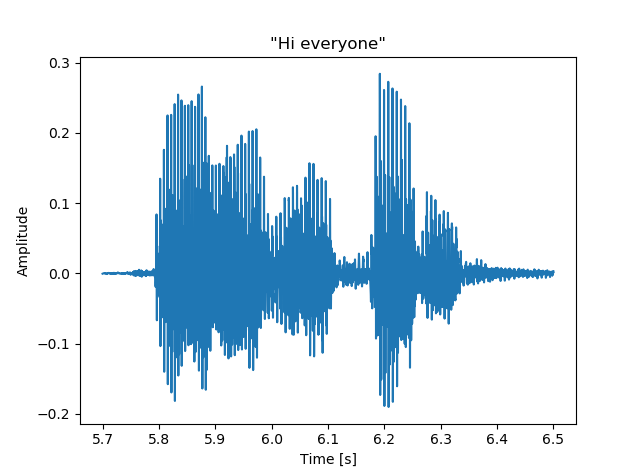
\includegraphics[scale=0.5]{res/audio_sig.png}
  \caption{Nasumichni noramlizovani audio signal iz baze}
  \label{fig:3}
  \vspace{0pt}
\end{figure}
\begin{figure}[!h]
        \centering
        \begin{subfigure}{0.475\textwidth}
            \centering
            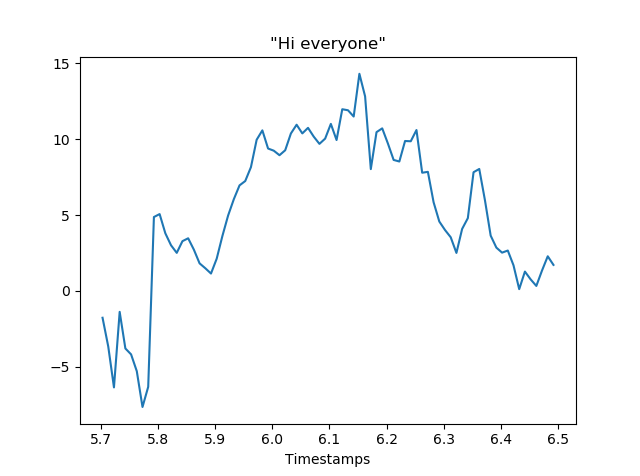
\includegraphics[scale=0.5]{res/cep1.png}
            \caption{Prvi MFKK}
            \label{fig:4a}
            \vspace{0pt}
        \end{subfigure}%
        \begin{subfigure}{0.475\textwidth}
            \centering
            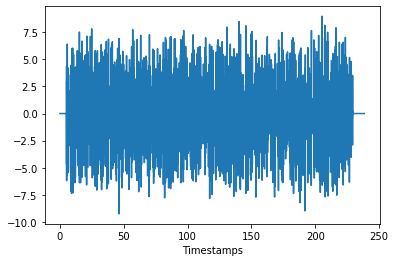
\includegraphics[scale=0.5]{res/Dcep1.png}
            \caption{Delta prvog MFKK}
            \label{fig:4b}
            \vspace{0pt}
        \end{subfigure}
        \caption{Prikaz glasovnih obelezhja}
        \label{fig:4}
\end{figure}
\newpage
\begin{figure}[!h]
        \centering
        \begin{subfigure}{0.475\textwidth}
            \centering
            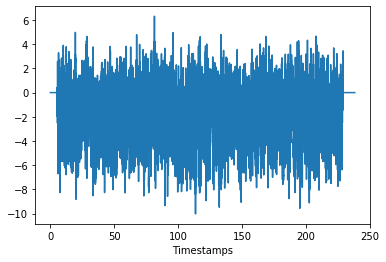
\includegraphics[scale=0.5]{res/cep6.png}
            \caption{Shesti MFKK}
            \label{fig:5a}
            \vspace{0pt}
        \end{subfigure}%
        \begin{subfigure}{0.475\textwidth}
            \centering
            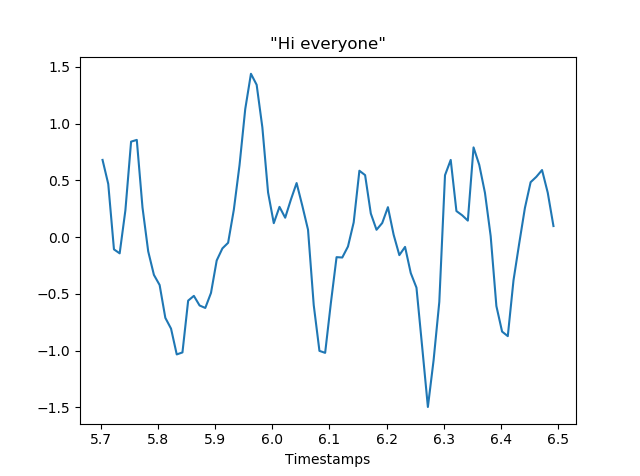
\includegraphics[scale=0.5]{res/Dcep6.png}
            \caption{Delta shestog MFKK}
            \label{fig:5b}
            \vspace{0pt}
        \end{subfigure}
        \caption{Prikaz glasovnih obelezhja}
        \label{fig:5}
\end{figure}
\begin{figure}[!h]
        \centering
        \begin{subfigure}{0.475\textwidth}
            \centering
            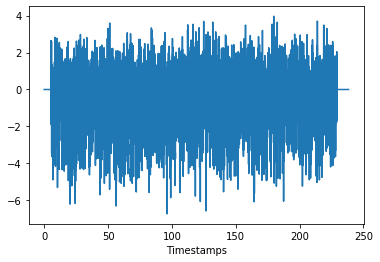
\includegraphics[scale=0.5]{res/cep12.png}
            \caption{Dvanaesti MFKK}
            \label{fig:6a}
            \vspace{0pt}
        \end{subfigure}%
        \begin{subfigure}{0.475\textwidth}
            \centering
            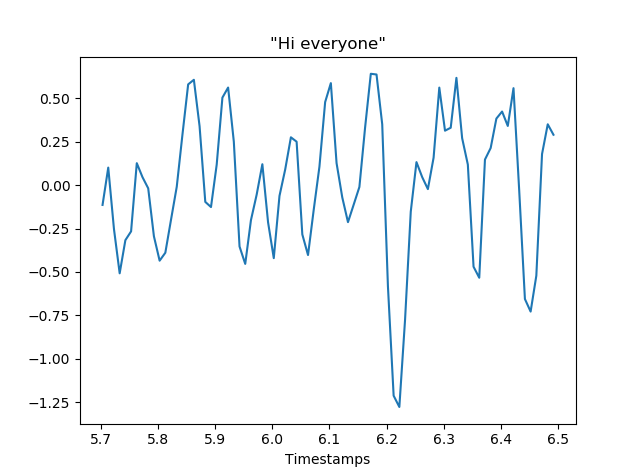
\includegraphics[scale=0.5]{res/Dcep12.png}
            \caption{Delta dvanaestog MFKK}
            \label{fig:6b}
            \vspace{0pt}
        \end{subfigure}
        \caption{Prikaz glasovnih obelezhja}
        \label{fig:6}
\end{figure}

\chapter{Obelezhja videa}

\chapter{Rekurentne neuralne mrezhe}

\chapter{Obuchavanje modela}

\chapter{Sinteza videa}


\begin{thebibliography}{99}

\bibitem{OPGpredavanja}
Djurovic1, Zh. Materijali sa predmeta Obrada i prepoznavanje govora
\bibitem{kepstrum} 
Delic1, V. Analiza mel-frekvencijskih kepstralnih koeficijenata kao obelezhja korish\-c1enih pri automat\-skom prepoznavanju govornika
\bibitem{MFKKlink}
\fontencoding{T1}\selectfont
\url{http://practicalcryptography.com/miscellaneous/machine-learning/guide-mel-frequency-cepstral-coefficients-mfccs/}
\bibitem{FFmpeg}
\url{https://ffmpeg.org/}
\bibitem{FFmpegN}
\url{https://github.com/slhck/ffmpeg-normalize}
\end{thebibliography}
\end{document}